\documentclass[tikz,border=10pt]{standalone}
\usepackage{tikz}
\usepackage{amsmath}
\usetikzlibrary{shapes.geometric, arrows.meta, positioning, fit, backgrounds}

\begin{document}
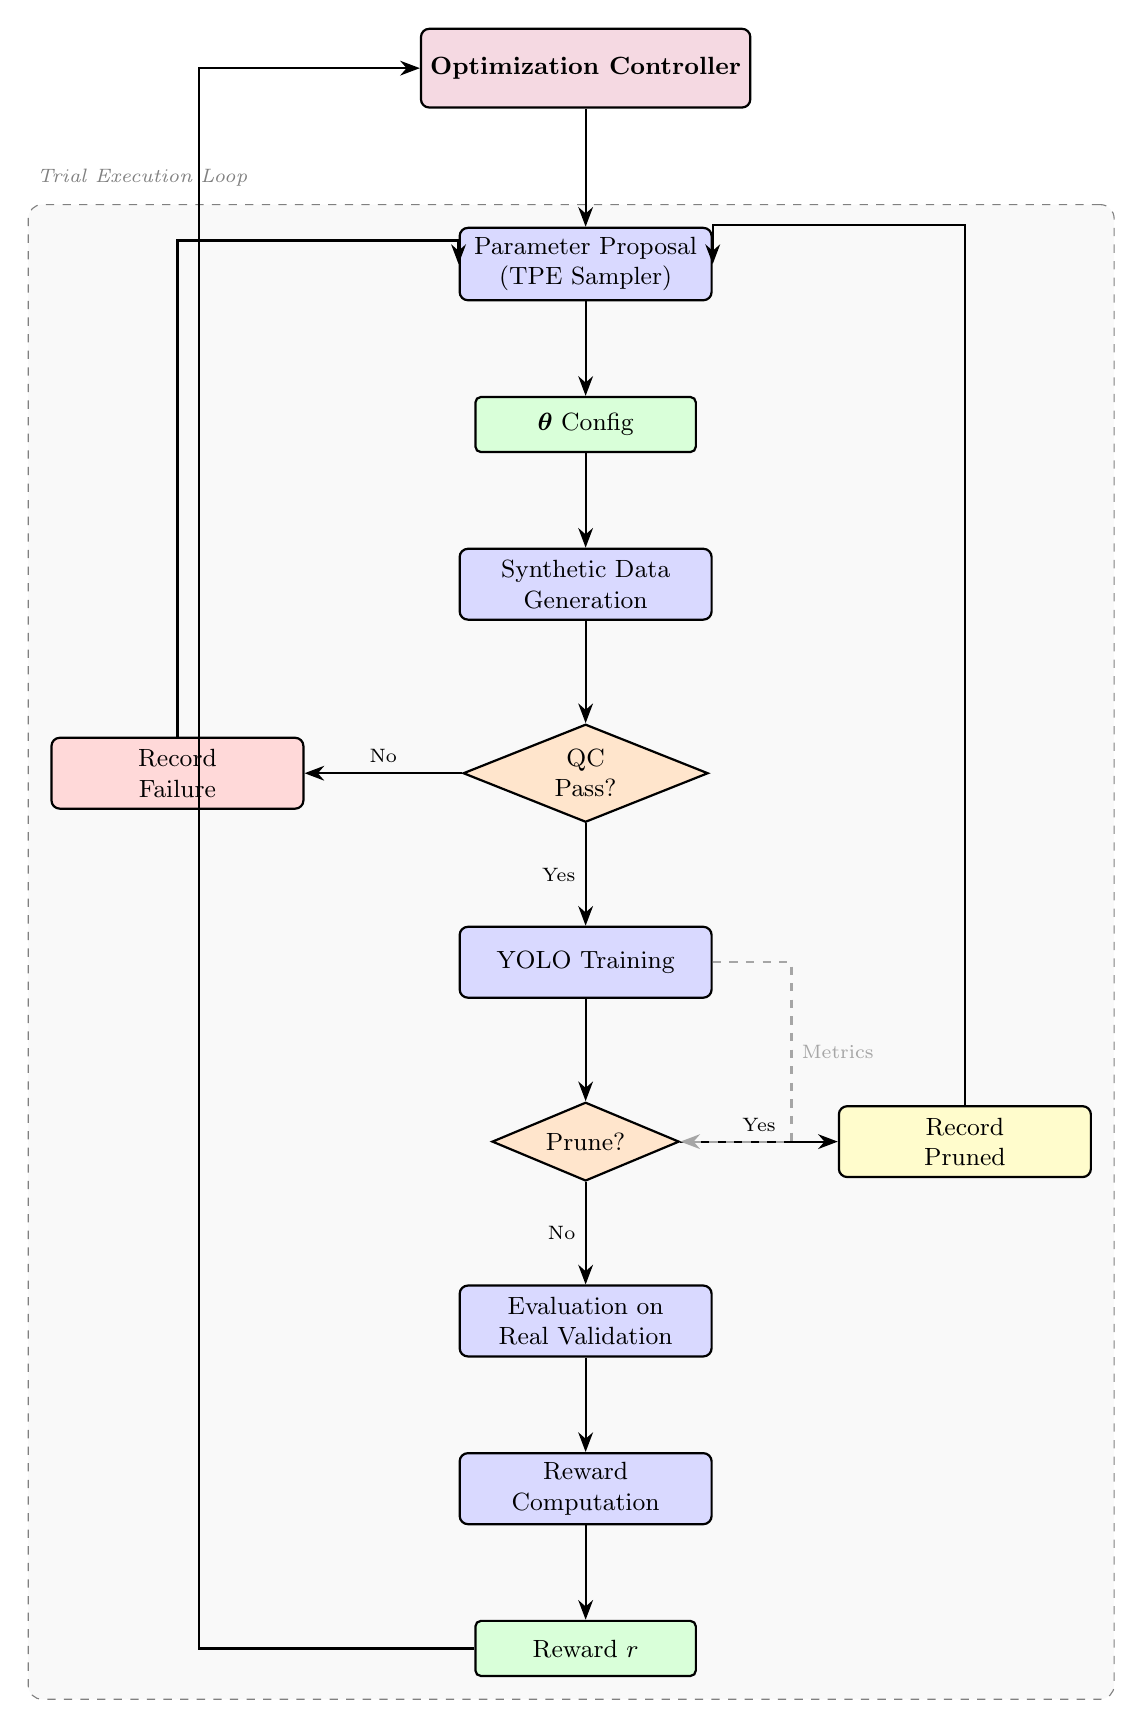
\begin{tikzpicture}[
    node distance=1.2cm and 1.8cm,
    process/.style={rectangle, draw=black, thick, fill=blue!15, minimum width=3.2cm, minimum height=0.9cm, align=center, rounded corners=3pt, font=\small},
    decision/.style={diamond, draw=black, thick, fill=orange!20, minimum width=1.5cm, minimum height=1cm, align=center, aspect=2.5, font=\small},
    data/.style={rectangle, draw=black, thick, fill=green!15, minimum width=2.8cm, minimum height=0.7cm, align=center, rounded corners=2pt, font=\small},
    controller/.style={rectangle, draw=black, thick, fill=purple!15, minimum width=3.5cm, minimum height=1cm, align=center, rounded corners=3pt, font=\small\bfseries},
    arrow/.style={-{Stealth[length=2.5mm]}, thick},
    dasharrow/.style={-{Stealth[length=2.5mm]}, thick, dashed, color=gray!70}
]

% Optimization Controller at top
\node[controller] (controller) {Optimization Controller};

% Main flow
\node[process, below=1.5cm of controller] (propose) {Parameter Proposal\\(TPE Sampler)};
\node[data, below=of propose] (params) {$\boldsymbol{\theta}$ Config};
\node[process, below=of params] (generate) {Synthetic Data\\Generation};
\node[decision, below=1.3cm of generate] (qc) {QC\\Pass?};

% Left branch for QC failure
\node[process, left=2cm of qc, fill=red!15] (fail) {Record\\Failure};

% Continue main flow
\node[process, below=1.3cm of qc] (train) {YOLO Training};
\node[decision, below=1.3cm of train] (prune) {Prune?};

% Right branch for pruning
\node[process, right=2cm of prune, fill=yellow!20] (pruned) {Record\\Pruned};

% Continue main flow
\node[process, below=1.3cm of prune] (eval) {Evaluation on\\Real Validation};
\node[process, below=of eval] (reward) {Reward\\Computation};
\node[data, below=of reward] (signal) {Reward $r$};

% Arrows for main flow
\draw[arrow] (controller) -- (propose);
\draw[arrow] (propose) -- (params);
\draw[arrow] (params) -- (generate);
\draw[arrow] (generate) -- (qc);
\draw[arrow] (qc) -- node[left, font=\scriptsize] {Yes} (train);
\draw[arrow] (train) -- (prune);
\draw[arrow] (prune) -- node[left, font=\scriptsize] {No} (eval);
\draw[arrow] (eval) -- (reward);
\draw[arrow] (reward) -- (signal);

% Failure branches
\draw[arrow] (qc) -- node[above, font=\scriptsize] {No} (fail);
\draw[arrow] (prune) -- node[above, font=\scriptsize] {Yes} (pruned);

% Feedback loops
\draw[arrow] (fail.north) |- ([yshift=0.3cm]propose.west) -- (propose.west);
\draw[arrow] (pruned.north) |- ([yshift=0.5cm]propose.east) -- (propose.east);
\draw[arrow] (signal.west) -- ++(-3.5,0) |- (controller.west);

% Intermediate metrics feedback to pruner
\draw[dasharrow] (train.east) -- ++(1,0) |- node[right, font=\scriptsize, pos=0.25] {Metrics} (prune.east);

% Background for main loop
\begin{scope}[on background layer]
    \node[draw=gray, dashed, rounded corners=5pt, fit=(propose)(signal)(fail)(pruned), inner sep=8pt, fill=gray!5] (loop) {};
\end{scope}

% Label
\node[above=0.1cm of loop.north west, anchor=south west, font=\scriptsize\itshape, color=gray] {Trial Execution Loop};

\end{tikzpicture}
\end{document}
